\renewcommand{\arraystretch}{1.5}
\begin{longtable}{
    |p{4cm}
    |p{5cm}
    |p{5cm}|
}
\caption{Comparativa de sensores para medición de conductividad eléctrica.}
\label{tab:sensor_conductividad} \\
\hline
\textbf{Característica} 
    & \textbf{Gravity: Analog EC Sensor V2 (DFR0300) \cite{DFRobot_EC_Sensor}} 
    & \textbf{Atlas Scientific EZO-EC™ \cite{AtlasScientific_Conductivity}} \\ 
\hline
\endfirsthead

\hline
\textbf{Característica} 
    & \textbf{Gravity: Analog EC Sensor V2 (DFR0300) \cite{DFRobot_EC_Sensor}} 
    & \textbf{Atlas Scientific EZO-EC™ \cite{AtlasScientific_Conductivity}} \\ 
\hline
\endhead

\hline
\multicolumn{3}{r}{\textit{Continúa en la siguiente página}} \\
\endfoot

\hline
\endlastfoot

Tipo de tecnología 
    & Electrodos de conductividad (K=1.0) 
    & Electrodos de conductividad \\ \hline

Parámetro principal 
    & Conductividad (EC) 
    & Conductividad (EC) \\ \hline

Rango de medición 
    & 0--20,000~$\mu$S/cm 
    & 0--200,000~$\mu$S/cm \\ \hline

Precisión 
    & $\pm$5\% F.S. 
    & $\pm$2\% F.S. \\ \hline

Tipo de salida 
    & Analógica (0--3.0 V) 
    & UART / I2C / Analógica \\ \hline

Voltaje de operación 
    & 3.0--5.0 V 
    & 3.3--5.5 V \\ \hline

Compatibilidad con ESP32 
    & Sí (ADC) 
    & Sí (UART/I2C/ADC) \\ \hline

Diseñado para monitoreo continuo 
    & Sí (recalibración periódica requerida) 
    & Sí (mínimo mantenimiento) \\ \hline

Vida útil de la sonda 
    & 6--12 meses 
    & $>$2 años \\ \hline

Calibración necesaria 
    & Periódica (solución estándar de conductividad) 
    & Muy baja frecuencia \\ \hline

Costo aproximado 
    & \$70 USD 
    & \$200+ USD \\ \hline

Ventajas 
    & Buen rango, estable, económico 
    & Alta precisión, muy robusto \\ \hline

Desventajas 
    & Requiere calibración manual periódica 
    & Alto costo, integración más compleja \\ \hline

Imagen
    & \shortstack{\\ 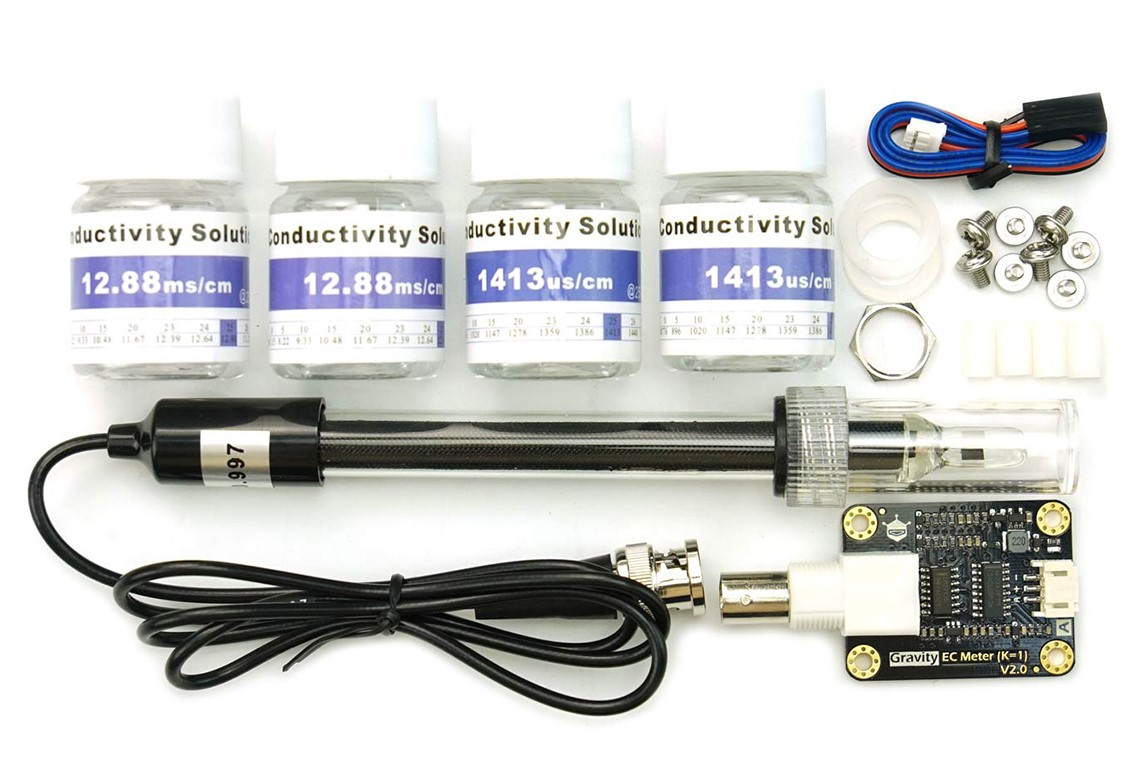
\includegraphics[width=0.8\linewidth]{Documento/Imagenes/Análisis/sensores/conductividad sensor.jpg}}
    & \shortstack{\\ 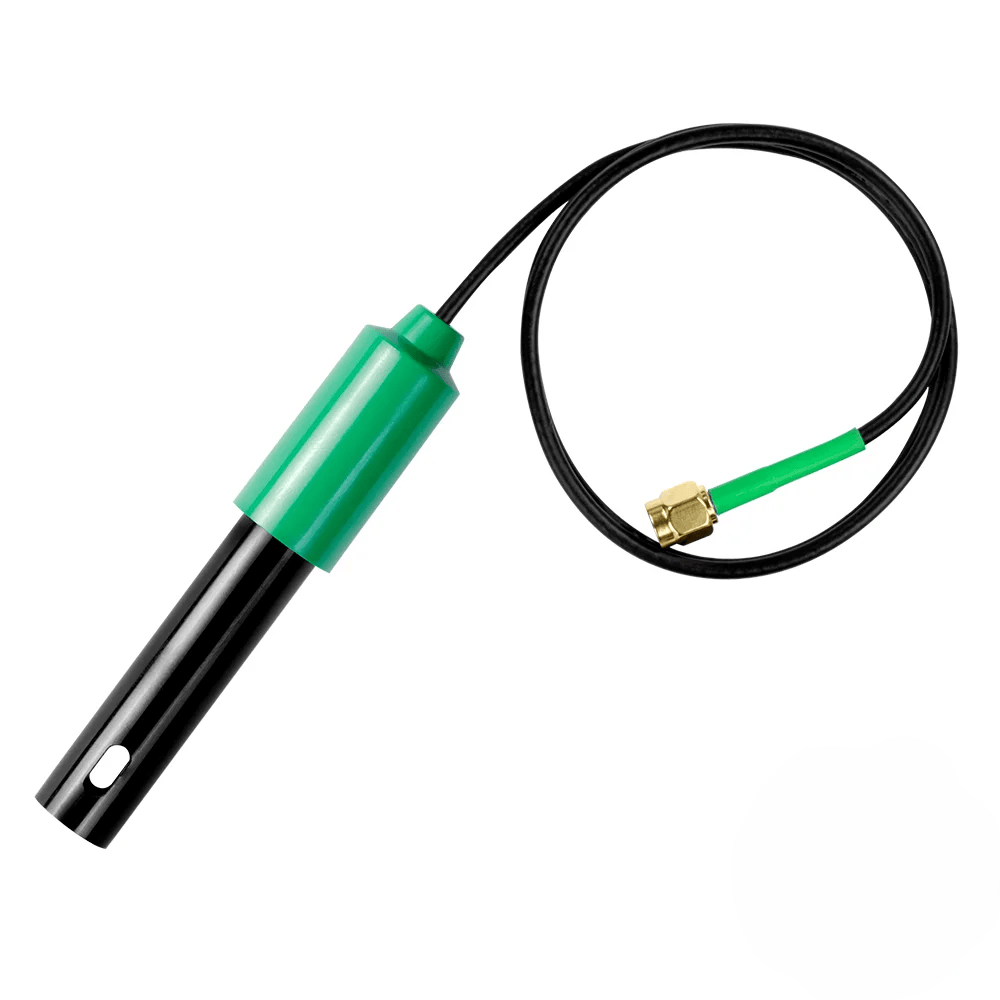
\includegraphics[width=0.8\linewidth]{Documento/Imagenes/Análisis/sensores/conductividad atlas sensor.png}} \\ \hline

\end{longtable}
